\begin{frame}{$d(K^-, n)"\pi^{\mp}\Sigma^{\pm}"$の分離}
  \begin{tabular}{cc}
    \begin{minipage}{0.5\hsize}
      \begin{figure}
        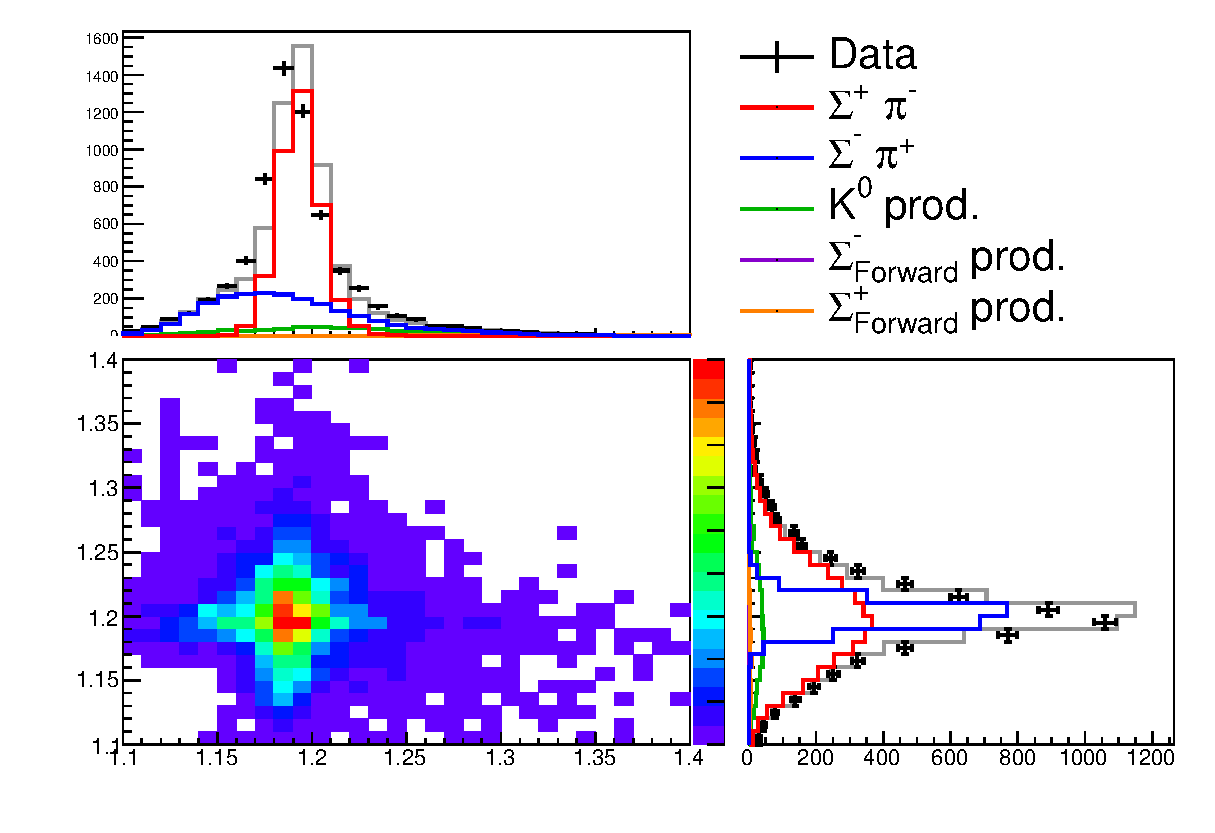
\includegraphics[width=4.5cm]{../pic/Run78/KN_ana_NC170_2sigma/KNpim_KNpip_MM.eps}
        \captionsetup{font=scriptsize}
        \caption{
          $d(K^-, n)"X"$のすべてのビンの足し合わせた図
        }
      \end{figure}
    \end{minipage}
    
    \begin{minipage}{0.5\hsize}
      \begin{itemize}
      \item $d(K^-, n)"\pi^-\Sigma^+"$\\
        \scriptsize
        $d(K^-, n \pi^-)"X"$では上図のように\\$\Sigma^+$にピーク\\
        $d(K^-, n \pi^+)"X"$では横図のように\\広く分布\\

      \item $d(K^-, n)"\pi^+\Sigma^-"$\\
        \scriptsize
        $d(K^-, n)"\pi^-\Sigma^+"$の電荷が反対。\\
      \end{itemize}
      \centering
      \tiny
      ビン毎はp.\pageref{page:fitKNpi},\pageref{page:fitKNpi2}参照
    \end{minipage}
  \end{tabular}

  \tminipageTwo{
    \begin{figure}
      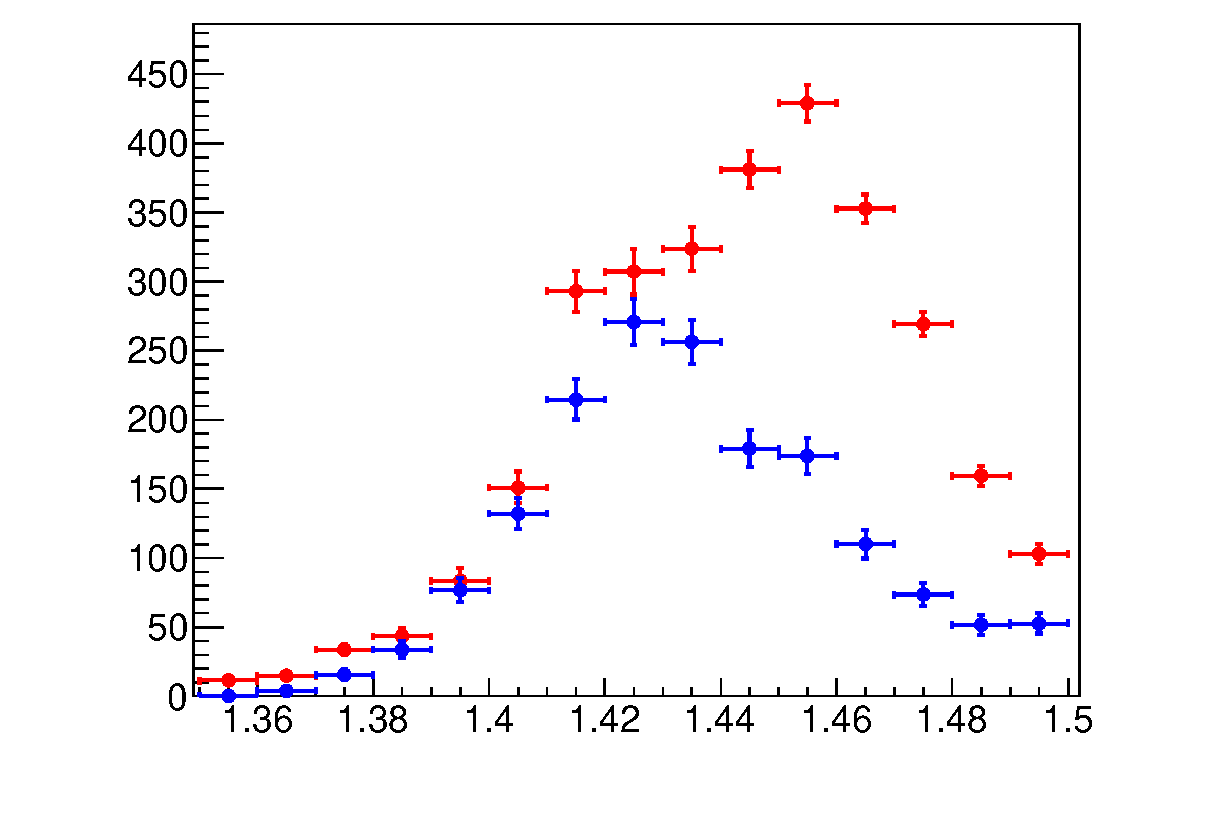
\includegraphics[width=4.5cm]{../pic/Run78/KN_ana_NC170_2sigma/piS_num.eps}
      \captionsetup{font=scriptsize}
      \caption{
        \centering
        $d(K^-, n \pi^{\mp})"\Sigma^{\pm}"$による$\pi^{\mp}\Sigma^{\pm}$の \protect\linebreak
        分離したカウント数
      }
    \end{figure}
  }{
    \begin{figure}
      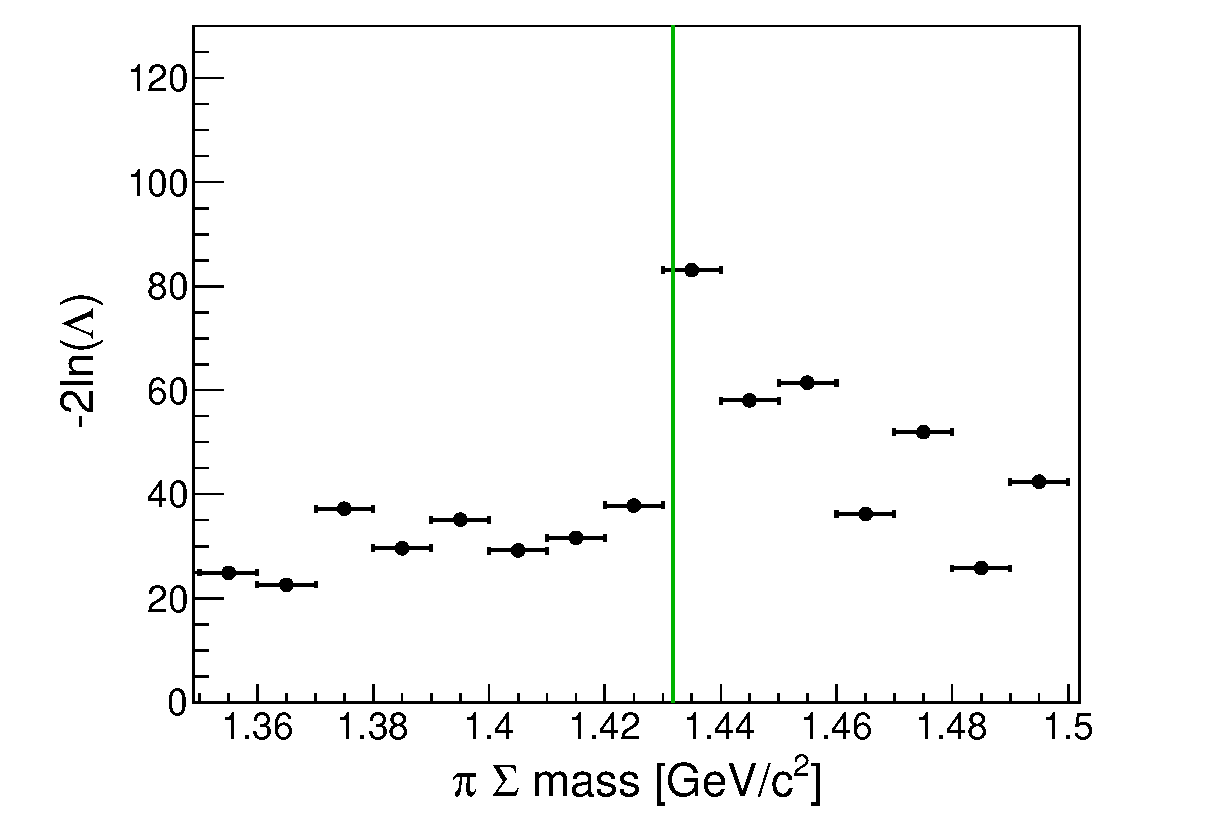
\includegraphics[width=4.5cm]{../pic/Run78/KN_ana_NC170_2sigma/Chi2.eps}
      \captionsetup{font=scriptsize}
      \caption{
        $d(K^-, n \pi^{\mp})"\Sigma^{\pm}"$フィッテイングの対数尤度
      }
    \end{figure}
  }
\end{frame}
